\documentclass{beamer}
\usepackage{beamerthemesplit}
\usepackage{wrapfig}
\usetheme{SPbGU}
\usepackage{pdfpages}
\usepackage{amsmath}
\usepackage{mathtools}
\usepackage{cmap} 
\usepackage[T2A]{fontenc} 
\usepackage[utf8]{inputenc}
\usepackage[english,russian]{babel}
\usepackage{indentfirst}
\usepackage{amsmath}
\usepackage{tikz}
\usepackage{multirow}
\usepackage[noend]{algpseudocode}
\usepackage{algorithm}
\usepackage{algorithmicx}
\usepackage{ stmaryrd }
\usepackage{qtree}
\usetikzlibrary{shapes,arrows}
\usepackage{fancyvrb}
\newtheorem{rutheorem}{Теорема}
\newtheorem{ruproof}{Доказательство}
\newtheorem{rudefinition}{Определение}
\newtheorem{rulemma}{Лемма}
\beamertemplatenavigationsymbolsempty

\newcommand{\derive}[0]{\xRightarrow[]{*}}
\newcommand{\derivek}[1]{\xRightarrow[]{#1}}
\newcommand{\deriveg}[1]{\xRightarrow[#1]{*}}
\newcommand{\derivegone}[1]{\xRightarrow[#1]{}}

\title[]{Теория автоматов и формальных языков}
\subtitle[]{Контекстно-свободные языки}
\institute[]{
Санкт-Петербургский государственный электротехнический университет <<ЛЭТИ>>\\
}

\author[]{Екатерина Вербицкая}

\date{11 октября 2016г.}

\definecolor{orange}{RGB}{179,36,31}

\begin{document}
{
  \begin{frame}
    \titlepage
  \end{frame}
}


\begin{frame}[fragile]
  \transwipe[direction=90]
  \frametitle{В предыдущей серии}
  \begin{itemize}
    \item Контекстно-свободные грамматики (все правила имеют вид $A \rightarrow \alpha$) 
    \item КС языки и разрешимость проверки пустоты
    \item Нормальная форма Хомского
    \item Алгоритм CYK
  \end{itemize}
\end{frame}

\begin{frame}[fragile]
  \transwipe[direction=90]
  \frametitle{В предыдущей серии: НФХ}
  КС грамматика находится в \textbf{нормальной форме Хомского}, если все ее правила имеют вид: 
  \begin{itemize}
    \item $A \rightarrow B C$, где $A,B,C \in V_N$
    \item $A \rightarrow a$, где $A \in V_N, a \in V_T$
    \item $S \rightarrow \varepsilon$, если в языке есть пустое слово, где $S$ --- стартовый нетерминал
  \end{itemize}

  \begin{enumerate}
    \item Удалить стартовый нетерминал из правых частей правил 
    \item Избавиться от неодиночных терминалов в правых частях 
    \item Удалить длинные правила (длины больше 2)
    \item Удалить непродуктивные правила ($\varepsilon$-правила)
    \item Удалить цепные правила
   \end{enumerate}
\end{frame}


\begin{frame}[fragile]
  \transwipe[direction=90]
  \frametitle{В предыдущей серии: CYK}
  \begin{itemize}
      \item Алгоритм синтаксического анализа, работающий с грамматиками в НФХ
      \item Динамическое программирование
  \end{itemize}

  \begin{center}
    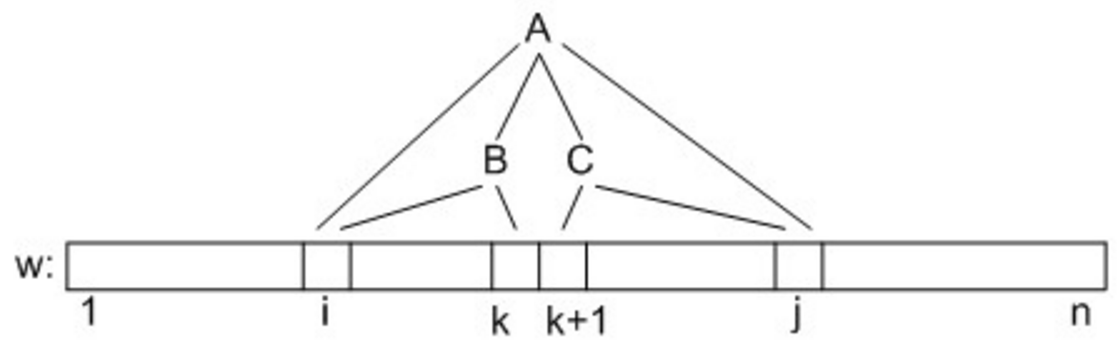
\includegraphics[width=\textwidth]{pics/CYK.png}  
  \end{center}
\end{frame}


\begin{frame}[fragile]
  \transwipe[direction=90]
  \frametitle{В предыдущей серии: CYK}
  \begin{itemize}
      \item Дано: строка $\omega$ длины $n$, грамматика $G = \langle V_T, V_N, P, S\rangle$ в НФХ
      \item Используем трехмерный массив d булевых значений размером $|V_N| \times n \times n$, $d[A][i][j] = true \Leftrightarrow A \derive \omega[i \dots j]$
      \item Инициализация: $i = j$
      \begin{itemize}
        \item $d[A][i][i] = true$, если в грамматике есть правило $A \rightarrow \omega[i]$
        \item $d[A][i][i] = false$, иначе
      \end{itemize}
      \item Динамика. Предполагаем, d построен для всех нетерминалов и пар $\{(i', j') \, | \, j' - i' < m \}$
      \begin{itemize}
        \item $d[A][i][j] = \bigvee_{A\rightarrow BC}^{}{\bigvee_{k=i}^{j-1}{d[B][i][k] \wedge d[C][k+1][j]}}$
      \end{itemize}
      \item В конце работы алгоритма в $d[S][0][n]$ записан ответ, выводится ли $\omega$ в данной грамматике
  \end{itemize}
\end{frame}

\begin{frame}[fragile]
  \transwipe[direction=90]
  \frametitle{Восходящий синтаксический анализ}
  \begin{itemize}
      \item Начинаем с символов входной строки, строим дерево вывода до стартового нетерминала
      \item CYK --- один из примеров восходящего синтаксического анализа
      \item Контринтуитивен 
  \end{itemize}
\end{frame}

\begin{frame}[fragile]
  \transwipe[direction=90]
  \frametitle{Нисходящий синтаксический анализ}
  \begin{itemize}
      \item Хотим построить левосторонний вывод строки
      \item Начинаем со стартового нетерминала, раскрываем нетерминалы до тех пор, пока не получим вывод строки
      \item Интуитивен
  \end{itemize}
\end{frame}

\begin{frame}[fragile]
  \transwipe[direction=90]
  \frametitle{Нисходящий синтаксический анализ: функция $FIRST$}
  \begin{itemize}
      \item Функция $FIRST^G_k(\alpha) = \{ \omega \in V_T^* \, |$ либо $|\omega| < k$ и $ \alpha \derive \omega$, либо $|\omega| = k$ и $\alpha \derive \omega \gamma, \gamma \in V_T^*\}$
      \begin{itemize}
        \item По сути: первые $k$ символов, встречающиеся в выводе из $\alpha$
      \end{itemize}
      \item Пример
      \begin{itemize}
        \item $S \rightarrow S S \, | \, a S b \, | \, \varepsilon$
        \item $FIRST^G_3( a S b ) = \{ ab, aab, aaa\} $
        \item $aba \notin FIRST^G_3 (a S b)$!
      \end{itemize}    
  \end{itemize}
\end{frame}


\begin{frame}[fragile]
  \transwipe[direction=90]
  \frametitle{Нисходящий синтаксический анализ: LL-грамматики}
    Фундаментальное свойство: по сентенциальной форме $a_1 a_2 \dots a_j A \beta, a_i \in V_T, A \in V_N, \beta \in (V_T \cup V_N)^*$ однозначно определяется, какое правило нужно применять дальше, чтобы разобрать всю строку \pause
    
    ~\\~
      
   КС грамматика $G$ является $\textbf{LL(k)}$\textbf{-грамматикой} для некоторого $k$,  если для любых двух левосторонних выводов вида 
  \begin{itemize}
    \item $S \derive \omega A \alpha \Rightarrow \omega \beta \alpha \derive \omega \delta$
    \item $S \derive \omega A \alpha \Rightarrow \omega \gamma \alpha \derive \omega \eta$
  \end{itemize}
  в которых $FIRST^G_k(\delta) = FIRST ^G_k(\eta)$, верно $\beta = \gamma$

~\\~

  КС грамматика $G$ является $\textbf{LL}$\textbf{-грамматикой}, если она является $LL(k)$-грамматикой для некоторого $k \geq 0$
\end{frame}


\begin{frame}[fragile]
  \transwipe[direction=90]
  \frametitle{Пример LL(1)-грамматики}
  $S \rightarrow a B S \, | \, b$
  
  $B \rightarrow a \, | \, b S B$

  Надо показать: для любых левосторонних выводов
  \begin{itemize}
    \item $S \derive \omega A \alpha \Rightarrow \omega \beta \alpha \derive \omega \delta$
    \item $S \derive \omega A \alpha \Rightarrow \omega \gamma \alpha \derive \omega \eta$
  \end{itemize} 
  если $\delta$ и $\eta$ начинаются с одного символа, то $\beta = \gamma$
  
  Рассматриваем выводы, где роль $A$ выполняет $S$: $S \Rightarrow a B S, S \Rightarrow b$. $\omega = \alpha = \varepsilon, \beta = a B S, \gamma = b$. Любая цепочка, выводимая из $\beta \alpha = a B S$ начинается на $a$; любая цепочка, выводимая из $\gamma \alpha = b$ начинается на $b$. Однозначно определяется, какой альтернативе следовать. 
  
  Аналогично с $A = B: S \Rightarrow a B S \Rightarrow a a S; S \Rightarrow a B S \Rightarrow a b S B S$ 
\end{frame}


\begin{frame}[fragile]
  \transwipe[direction=90]
  \frametitle{Простая LL(1)-грамматика}
  КС-грамматика $G$ называется \textbf{простой LL(1)-грамматикой}, если в ней нет $\varepsilon$-правил, и все альтернативы для каждого нертерминала начинаются с терминалов, и притом различных. 
  
  ~\\~ 
  
  $\forall (A, a), A \in V_N, a \in V_T, \exists $ самое большое 1 альтернатива вида $A \rightarrow a \alpha$
  
\end{frame}


\begin{frame}[fragile]
  \transwipe[direction=90]
  \frametitle{LL-грамматика: необходимое и достаточное условие}
  \begin{rutheorem}
  КС грамматика $G = \langle V_N, V_T, P, S \rangle$ является $LL(k)$-грамматикой $\Leftrightarrow FIRST^G_k(\beta \alpha) \cap FIRST^G_k(\gamma \alpha) = \varnothing$, для всех таких $\alpha, \beta, \gamma: A \rightarrow \beta, A \rightarrow \gamma \in P, \beta \neq \gamma, \exists$ вывод $S \derive \omega A \alpha$
  \end{rutheorem}  

\end{frame}

\begin{frame}[fragile]
  \transwipe[direction=90]
  \frametitle{LL-грамматика: функция FOLLOW}
  $FOLLOW^G_k(\beta) = \{ \omega \in V_T^* \, | \, S \derive \gamma \beta \alpha, \omega \in FIRST^G_k(\alpha) \}, k \geq 0$

  ~\\~
  
   Пример: $S \rightarrow S S \, | \, a S b \, | \, \varepsilon$
   
   \begin{itemize}
     \item  $FOLLOW^G_3( a a ) = \{ a b b, a a b, a a a, a b a, b a a, b a b, b b, b b a, \dots \}$
     \item $\varepsilon, b \notin FOLLOW^G_3$!
   \end{itemize}
\end{frame}


\begin{frame}[fragile]
  \transwipe[direction=90]
  \frametitle{LL(1)-грамматика: необходимое и достаточное условие}
  \begin{rutheorem}
    КС-грамматика  $G = \langle V_N, V_T, P, S \rangle$ является $LL(1)$-грамматикой $\Leftrightarrow FIRST^G_1 (\beta FOLLOW^G_1(A)) \cap FIRST^G_1(\gamma FOLLOW^G_1(A)) = \varnothing, \forall A \in V_N, \beta, \gamma \in (V_N \cup V_T)^*, A \rightarrow \gamma, A \rightarrow \beta \in P, \beta \neq \gamma$
  \end{rutheorem}
  
\end{frame}

\begin{frame}[fragile]
  \transwipe[direction=90]
  \frametitle{LL(1)-грамматика: необходимое и достаточное условие: другая формулировка}
  \begin{rutheorem}
    КС-грамматика  $G = \langle V_N, V_T, P, S \rangle$ является $LL(1)$-грамматикой $\Leftrightarrow 
    \forall A \rightarrow \alpha_1 \, | \, \alpha_2 \, | \, \dots \, | \, \alpha_n$ верно: 
    \begin{itemize}
      \item $FIRST^G_1(\alpha_i) \cap FIRST^G_1(\alpha_j) = \varnothing, i \neq j, 1 \leq i, j \leq n$
      \item если $\alpha_i \derive \varepsilon,$ то $FIRST^G_1(\alpha_j) \cap FOLLOW^G_1(A) = \varnothing, 1 \leq j \leq n, i \neq j$
    \end{itemize}
   \end{rutheorem}
  
\end{frame}


\begin{frame}[fragile]
  \transwipe[direction=90]
  \frametitle{Леворекурсивность}
  \begin{rutheorem}
    Если  КС-грамматика  $G = \langle V_N, V_T, P, S \rangle$ леворекурсивна, то она не является $LL(k)$-грамматикой ни при каком $k$
  \end{rutheorem}
\end{frame}

 
   \end{document}
 

  
